\documentclass[conference]{IEEEtran}
\IEEEoverridecommandlockouts
% The preceding line is only needed to identify funding in the first footnote. If that is unneeded, please comment it out.
\usepackage{cite}
\usepackage{amsmath,amssymb,amsfonts}
\usepackage{algorithmic}
\usepackage{textcomp}
% \usepackage{latex-dev}
\usepackage{theorem,caption,extarrows,mathrsfs,physics,bm}
\usepackage{graphicx,xcolor,booktabs,subfigure,tikz}
\usepackage{pgfplots,grffile}
\usepackage{fontspec}
\usepackage[skins]{tcolorbox}
\setmainfont{CMU Serif}
\setsansfont{CMU Sans Serif}
\setmonofont{Sarasa Fixed SC Nerd Font}
\pgfplotsset{compat=newest}
%% the following commands are needed for some matlab2tikz features
\usetikzlibrary{plotmarks}
\usetikzlibrary{arrows.meta}
\usetikzlibrary{calc}
\usepgfplotslibrary{patchplots}
\def\BibTeX{{\rm B\kern-.05em{\sc i\kern-.025em b}\kern-.08em
T\kern-.1667em\lower.7ex\hbox{E}\kern-.125emX}}
%% Define the theorem and proof
\newtheorem{theorem}[subsection]{Theorem}
\newtheorem{definition}[subsection]{Definition}
\newenvironment{thmbox}{\par
\vspace{4pt}
\begin{center}
	\tcbset{enhanced,notitle,colframe=black,colback=white}
	\begin{tcolorbox}[fuzzy shadow={1.6mm}{-1.6mm}{0mm}{0mm}{fill=black!90!white},arc=0mm]}{\end{tcolorbox}
\end{center}}
\usepackage{listings}
\lstset{
    basicstyle          =   \sffamily,          % 基本代码风格
    keywordstyle        =   \bfseries,          % 关键字风格
    commentstyle        =   \rmfamily\itshape,  % 注释的风格,斜体
    stringstyle         =   \ttfamily,  % 字符串风格
    flexiblecolumns,                % 别问为什么,加上这个
    numbers             =   left,   % 行号的位置在左边
    showspaces          =   false,  % 是否显示空格,显示了有点乱,所以不现实了
    numberstyle         =   \tiny\ttfamily,    % 行号的样式,小五号,tt等宽字体
    showstringspaces    =   false,
    captionpos          =   t,      % 这段代码的名字所呈现的位置,t指的是top上面
    frame               =   shadowbox,   % 显示边框
    rulesepcolor=\color{red!20!green!20!blue!20}
}

\lstdefinestyle{Python}{
    language        =   Python, % 语言选Python
    backgroundcolor=\color{backpycol},
    basicstyle      =   \ttfamily,
    numberstyle     =   \ttfamily,
    keywordstyle    =   \color{blue},
    keywordstyle    =   [2] \color{teal},
    stringstyle     =   \color{magenta},
    commentstyle    =   \color[HTML]{338AAF}\ttfamily,
    breaklines      =   true,   % 自动换行,建议不要写太长的行
    columns         =   fixed,  % 如果不加这一句,字间距就不固定,很丑,必须加
    basewidth       =   0.5em,
}
\definecolor{codegreen}{rgb}{0,0.6,0}
\definecolor{codegray}{rgb}{0.5,0.5,0.5}
\definecolor{codepurple}{rgb}{0.58,0,0.82}
\definecolor{backcolour}{rgb}{0.95,0.95,0.92}
\definecolor{backpycol}{rgb}{0.97,0.95,0.97}
\lstdefinestyle{C++}{
    language =[ANSI]C,
    backgroundcolor=\color{backcolour},
    commentstyle=\color[HTML]{338AAF}\ttfamily,
    keywordstyle=\sffamily\bfseries\color{magenta},
    numberstyle=\color{codegray},
    stringstyle=\color{codepurple},
    basicstyle=\ttfamily,
    breakatwhitespace=false,
    breaklines=true,
    basewidth=0.5em,
    captionpos=b,
    columns=fixed,
    frame=shadowbox,
    keepspaces=true,
    numbers=left,
    numbersep=5pt,
    showspaces=false,
    showstringspaces=false,
    showtabs=false,
    tabsize=4
}
\lstdefinestyle{matlab}{
    language=matlab,
    backgroundcolor=\color{backcolour},
    commentstyle=\color[HTML]{338AAF}\ttfamily,
    keywordstyle=\sffamily\bfseries\color{magenta},
    numberstyle=\color{codegray},
    stringstyle=\color{codepurple},
    basicstyle=\ttfamily,
    breakatwhitespace=false,
    breaklines=true,
    basewidth=0.5em,
    captionpos=b,
    columns=fixed,
    keepspaces=true,
    numbers=left,
    numbersep=5pt,
    showspaces=false,
    showstringspaces=false,
    showtabs=false,
    tabsize=4,
    frame=shadowbox
}
\definecolor{mygreen}{rgb}{0,0.6,0}
\definecolor{mygray}{rgb}{0.5,0.5,0.5}
\definecolor{mymauve}{rgb}{0.58,0,0.82}
\definecolor{bggray}{rgb}{0.93,0.95,0.94}
\lstdefinestyle{pseudocode}{
    backgroundcolor=\color{bggray},
    columns=fullflexible,
    tabsize=4,
    breaklines=true,               % automatic line breaking only at whitespace
    captionpos=b,                  % sets the caption-position to bottom
    commentstyle=\color{mygreen},  % comment style
    escapeinside={\%*}{*)},        % if you want to add LaTeX within your code
    keywordstyle=\color{blue},     % keyword style
    stringstyle=\color{mymauve}\ttfamily,  % string literal style
    frame=shadowbox,
    rulesepcolor=\color{red!20!green!20!blue!20},
    % identifierstyle=\color{red},
    language=c++,
    numbers=left,
    numberstyle=\small\color{codegray},
    basicstyle=\ttfamily,% size of fonts used for the code
    escapeinside=``,
    xleftmargin=0.6em,
    xrightmargin=0.6em,
    aboveskip=1em
}
\lstdefinestyle{Fortran}{
    language =fortran,
    backgroundcolor=\color{backcolour},
    commentstyle=\color[HTML]{338AAF}\ttfamily,
    keywordstyle=\sffamily\bfseries\color{magenta},
    numberstyle=\small\color{codegray},
    stringstyle=\color{codepurple},
    basicstyle=\ttfamily,
    breakatwhitespace=false,
    breaklines=true,
    basewidth=0.5em,
    captionpos=b,
    columns=fixed,
    frame=shadowbox,
    keepspaces=true,
    numbers=left,
    numbersep=5pt,
    showspaces=false,
    showstringspaces=false,
    showtabs=false,
    tabsize=4
}

\title{EE332 Lab2: Simulation of Full Adder on Nexys 4 DDR}
\author{
	\IEEEauthorblockN{1\textsuperscript{st} Qiu Kunyuan}
	\IEEEauthorblockA{
		\textit{EEE. Southern University of Science and Technology}\\
		Shenzhen, PRC\\
		11913019@mail.sustech.edu.cn
	}
}
\begin{document}
\maketitle
% !TEX root=./index.tex

\begin{abstract}
	This report focuses on the phenomenons encountered in the simulation of a simple full adder, to reveal some critical features of FPGA programming comparing to ordinary programmable devices. Among these phenomenons, jitters and the race-hazard conditions are of the most concerns.
\end{abstract}
\vspace{1em}
\begin{IEEEkeywords}
	FPGA, programmable logic, full adder, race-hazard condition, jitter, delay
\end{IEEEkeywords}

\section{Introduction}

Half adder and full adder are basic elements in digital circuits used to perform addition operations on binary numbers.

A half adder

\begin{figure}[htpb]
	\begin{center}
		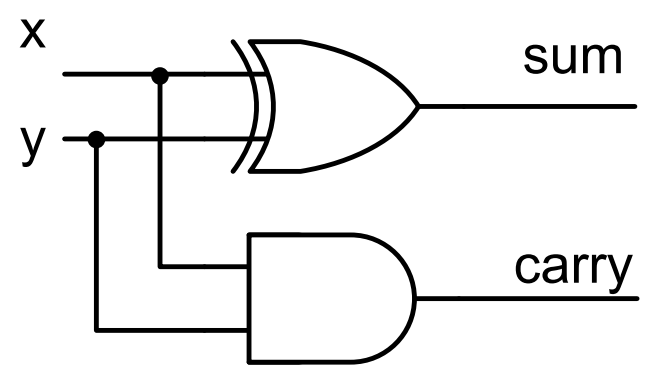
\includegraphics[width=0.22\textwidth]{index.assets/20240303235723.png}
		\caption{Gate Level Description of Half Adder}
	\end{center}
\end{figure}

is a combinational logic circuit that takes two binary inputs and produces two binary outputs: sum and carry.

\begin{eqnarray}
	\mathop{\mathrm{HA}}:(x_1,x_2)\mapsto(Q,C) :=
	\begin{cases}
			Q&=\mathop{\mathrm{xor}}(x_1,x_2) \\
			C&=\mathop{\mathrm{and}}(x_1,x_2)
	\end{cases}
\end{eqnarray}

The main limitation of the half adder is that it cannot handle carry inputs and therefore can only be used for 1-bit addition.

A full adder

\begin{figure}[htpb]
	\begin{center}
		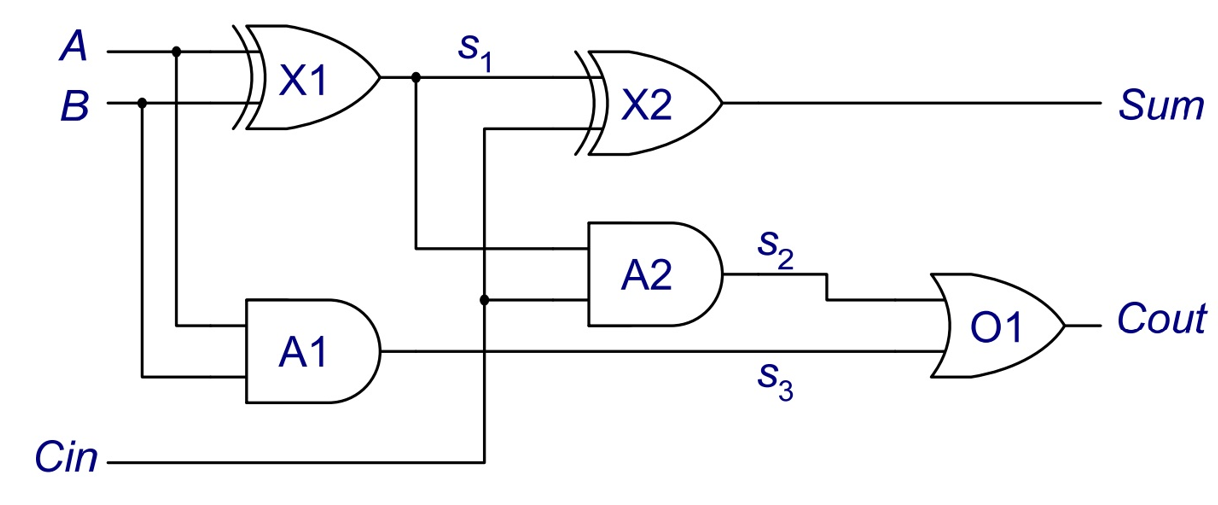
\includegraphics[width=0.45\textwidth]{index.assets/20240303235337.png}
		\caption{Gate Level Description of Full Adder}
	\end{center}
\end{figure}\label{FA_GateLevel}

is an extension of the half adder that accepts three binary inputs: two additions and a rounding input, and produces two binary outputs: sum and carry. Full adders can be connected in series to achieve binary addition of any number of bits.

Implementation of full adder can be derived directly from 3-digit addition, where the final carry output is toggled if any of \(X_1+X_2\) or \(C_i+Q_1\) produces a carry:

\begin{eqnarray}
	(q_1,c_1)&=\mathop{\mathrm{HA}}(x_1,x_2) \\
	(q_2,c_2)&=\mathop{\mathrm{HA}}(q_1,c_i) \\
	c_o &= \mathop{\mathrm{or}}(c_1,c_2)
\end{eqnarray}

Therefore the gate-level circuit of the full adder can be easily captured, as shown of Figure. (\ref{FA_GateLevel})

\section{Verilog Modeling}

There are two levels of HDL modeling for full adder, one for gate level description and one for behavioral level description.

\subsection{Gate-Level Implementation}

For the gate level modeling, the DNF (OR-AND) of the output ports are required:

\begin{eqnarray}
\begin{aligned}
	Q_2&=HA(HA(x_1,x_2)[0],c_i)[0] \\
	&=\mathop{\mathrm{xor}}(\mathop{\mathrm{xor}}(x_1,x_2),c_i) \\
	&= \overline{AB} C+\overline{A} B \overline{C} + A \overline{BC} +ABC \\
	C_{\mathrm{out}}&=AB+BC+AC
\end{aligned}
\end{eqnarray}

Therefore, the Verilog code is pretty straight forward:

\lstinputlisting[caption={Gate Level Modeling of Full Adder in Verilog}, language=verilog, style=verilog, label={glm_fa}, linewidth=0.92\linewidth]{../../lab2/lab2.srcs/sources_1/new/full_adder_g.v}
\end{document}